\chapter{Diseño del sistema} \label{chp:design}

En este capítulo se detalla el diseño del sistema, especificando a alto nivel cada parte que lo compone, incluyendo, también, esquemas que ilustran su estructura. Concretamente, se describirán las bibliotecas de \textit{\textbf{shaders}} \ref{sec:lib-shaders}, \textbf{errores} \ref{sec:lib-errors}, código \textbf{misceláneo } \textit{C} \ref{sec:lib-misc-c}, \textbf{polígonos} \ref{sec:lib-polygon} y \textbf{animaciones} \ref{sec:lib-animation}. En cada una de estas secciones, se tratan las decisiones de diseño tomadas respecto a cada biblioteca donde se expone cada elemento de la biblioteca y unas directrices sobre cómo utilizarlas desde la perspectiva del usuario.

\section{Leyenda}

La figura \ref{fig:lib-legend} es la leyenda que representa los elementos con los que se describe el sistema en los próximos diagramas de bibliotecas.

A continuación, se describen los diferentes componentes de sistema acompañados de diagramas que indican los elementos que lo componen y su relación:
\begin{itemize}
    \item \textbf{Lista azul}: indica una estructura de datos.
    \item \textbf{Lista verde}: indica un tipo \textbf{enumerado}.
    \item \textbf{Rectángulo}: indica una función o \textit{macro} 
    \item \textbf{Flechas}: indican la dependencia entre elementos, de forma que el elemento origen es la dependencia del elemento destino.
\end{itemize}

En los sucesivos apartados, se describen cada uno de los módulos que componen el sistema, comenzando por la biblioteca de \textit{shaders}. La figura \ref{fig:libraries-overview} muestra la estructura general de las bibliotecas empleadas en el proyecto y las relaciones de dependencia entre ellas.

\begin{figure}[htp]
    \centering
    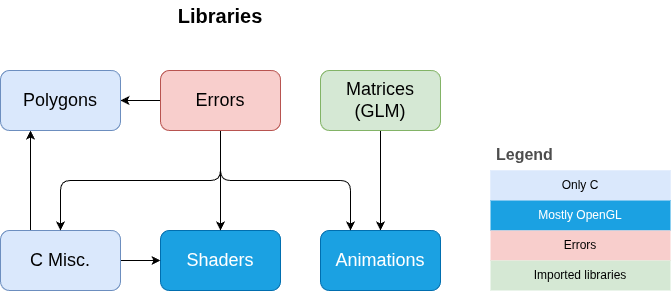
\includegraphics[width=0.9\textwidth]{figures/diagrams/libraries.png}
    \caption{Diagrama general de las bibliotecas y sus relaciones.}
    \label{fig:libraries-overview}
\end{figure}

\begin{figure}[htp]
    \centering
    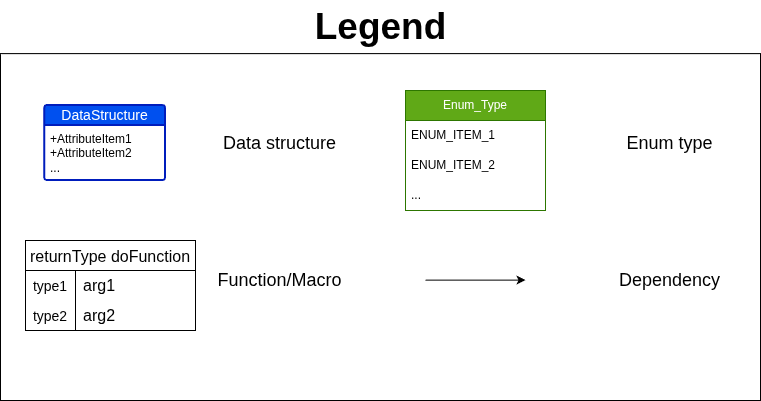
\includegraphics[width=0.7\textwidth]{figures/diagrams/libraries_legend.png}
    \caption{Leyenda de los diagramas de las bibliotecas.}
    \label{fig:lib-legend}
\end{figure}

\section{Shaders} \label{sec:lib-shaders}

En esta sección se trata la biblioteca de \textit{shaders}: su motivación, funciones, estructuras de datos y la \textit{API} pública que ofrece. En la figura \ref{fig:graph-libraries-shader} se representa la estructura de la biblioteca de \textit{shaders}, la cual existe con el propósito de facilitar el procesamiento de los mismos, en lugar de manualmente repetir el proceso cada vez que se deseen usar. Así, no es necesario leer, compilar y enlazar los \textit{shaders} manualmente.

\begin{figure}[htp]
    \centering
    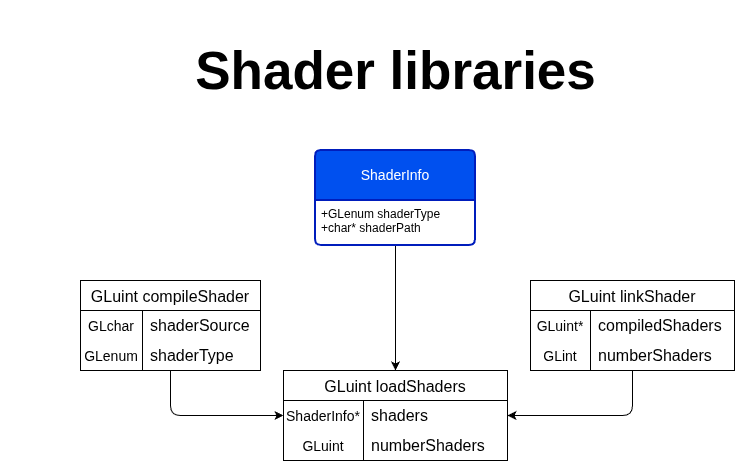
\includegraphics[width=0.9\textwidth]{figures/diagrams/libraries_shader.png}
    \caption{Diagrama de la biblioteca de shaders.}
    \label{fig:graph-libraries-shader}
\end{figure}

\subsection{Decisiones de diseño}

\lstinputlisting[
    float,
    floatplacement=!htp,
    language=C,
    label=cod:headers-shader-libraries,
    caption=Prototipos de la biblioteca de shaders
]{code/h_shader_libraries.h}

El código \ref{cod:headers-shader-libraries} muestra el prototipo de la biblioteca en código \textit{C}.

\begin{itemize}

    \item La estructura \textit{ShaderInfo} contiene el tipo del \textit{shader} y una cadena de caracteres contenido la ruta hacia el shader.
    
    \item Se ha separado el proceso del \textit{shader} en dos funciones que los compilan y enlazan en un programa: \textit{compileShader} y \textit{linkShader}. Luego, se utilizan las dos juntas en la función \textit{loadShader} junto a los datos recibidos en la estructura \textit{ShaderInfo}. De esta manera, en lugar de una sóla función con muchos argumentos que realice muchas tareas, se divide en varias partes y cooperan entre ellas.
    \begin{enumerate}
        \item La función \textit{compileShader} toma el contenido y el tipo del \textit{shader} para luego compilarlo. Devuelve su identificador como número entero sin signo.

        \item La función \textit{linkShader} toma una lista de \textit{shaders} compilados, es decir, sus identificadores, y los enlaza creando un programa. Devuelve su identificador como número entero sin signo.

        \item La función \textit{loadShaders} toma una lista de \textit{ShaderInfo} y los procesa utilizando las dos funciones anteriores, generando un programa. Para cada \textit{shader}, lee su contenido del fichero en la ruta correspondiente y lo compila según el tipo; los dos datos proporcionados por \textit{ShaderInfo}. Una vez compilados todos, se enlazan en un sólo programa. Devuelve su identificador como número entero sin signo.
        
    \end{enumerate}
    
\end{itemize}

\subsection{API pública}
El usuario deberá utilizar \textit{ShaderInfo}, completándola con los datos del tipo del \textit{shader} y su contenido en forma de cadena de caracteres. Posteriormente, llamar a la función \textit{loadShader} recibiendo estos datos; aunque se deja libertad para realizar el proceso manualmente, pudiendo llamar por separado a \textit{compileShader} y \textit{linkShader}.

\begin{itemize}
    \item Funciones internas:
    \begin{itemize}
        \item \textit{compileShader}.
        \item \textit{linkShader}.
    \end{itemize}
    
    \item Funciones públicas:
    \begin{itemize}
        \item \textit{loadShader}.
    \end{itemize}
    
    \item Estructuras públicas:
    \begin{itemize}
        \item \textit{ShaderInfo}.
    \end{itemize}
\end{itemize}

\section{Errores} \label{sec:lib-errors}

En esta sección se trata la biblioteca de \textbf{errores}: su motivación, funciones, estructuras de datos y la \textit{API} pública que ofrece. La figura \ref{fig:graph-libraries-error} representa la biblioteca de errores, que tiene como objetivo comprobar si el valor recibido es adecuado y proporcionar mensajes de error, a la vez que devuelve un número que indica si fue válido o no. De esta manera, se centralizan los errores y se reduce la comprobación caótica de ellos en el código. También, sería sencillo determinar qué tipo de error se intenta comprobar al revisar el código.

\begin{figure}[htp]
    \centering
    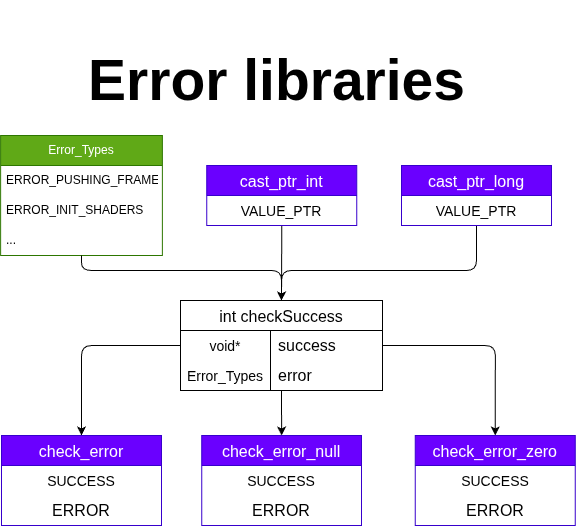
\includegraphics[width=0.9\textwidth]{figures/diagrams/libraries_error.png}
    \caption{Diagrama de la biblioteca de errores.}
    \label{fig:graph-libraries-error}
\end{figure}

\subsection{Decisiones de diseño}

\lstinputlisting[
    float,
    floatplacement=!htp,
    language=C,
    label=cod:headers-errors-libraries,
    caption=Prototipos de la biblioteca de errores
]{code/h_errors_libraries.h}

El código \ref{cod:headers-errors-libraries} muestra el prototipo de la biblioteca en código \textit{C}.

\begin{itemize}

    \item Se recopilan los tipos de errores en un enumerado llamado \textit{Error\_Types}: se organizan mediante texto y se traducen a números. De esta forma, es fácil distinguir qué error se pretende comprobar sin perder eficiencia.

    \item La función principal es \textit{checkSuccess}, que comprueba la validez de un valor según un tipo de error. Se utilizan también funciones \textit{macro} auxiliares para convertir tipos y retornar.
    \begin{enumerate}
    
        \item La función \textit{checkSuccess} toma una dirección a un valor y el tipo de error que se quiere comprobar, con el que se decide a qué tipo se debe transformar el valor y qué condición evaluar. De esta forma, puede determinarse qué tipo es el valor original sin crear demasiadas funciones. Por supuesto, conllevaría sus riesgos, concretamente en el mal uso del usuario al enviar los datos. Devuelve 0 en éxito y 1 en fracaso.

        \item Las funciones \textit{macro} \textit{cast\_ptr\_int} y \textit{cast\_ptr\_long} toman una dirección a un valor y devuelven ese mismo valor convertido al tipo \textit{int} o \textit{long}, respectivamente.

        \item En el caso de que se desee retornar un valor y finalizar la función en caso de que sea inválido, se han diseñado unas funciones \textit{macro} que comprueban la salida de \textit{checkSuccess} y devuelven un valor deseado: \textit{check\_error}, \textit{check\_error\_null}, \textit{check\_error\_zero}, que devuelven negativo, nulo y cero, respectivamente.
        
    \end{enumerate}

\end{itemize}

\subsection{API pública}
El usuario debería, tras una función crítica, comprobar el valor, ya sea llamando a alguna de las \textit{macros} o \textit{checkSuccess}, dependiendo de si se quiere devolver un valor o no.

\section{Misceláneo} \label{sec:lib-misc-c}

En esta sección se detalla la biblioteca de funciones \textbf{misceláneas}: su motivación, funciones, estructuras de datos y la \textit{API} pública que ofrece.

En la biblioteca miscelánea de \textit{C} \ref{fig:graph-libraries-miscc} se reúnen funciones auxiliares no dirigidas especialmente a \textit{OpenGL} y compuestas por código \textit{C} sin dependencias. Principalmente, se ha diseñado con la intención de ser utilizada para la lectura de ficheros, la creación de estructuras de datos y otras cuestiones generales de programación en \textit{C}.

\begin{figure}[htp]
    \centering
    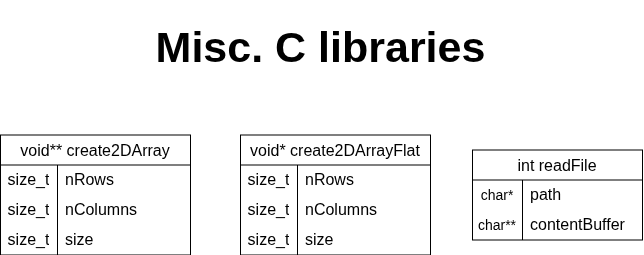
\includegraphics[width=1.0\textwidth]{figures/diagrams/libraries_miscc.png}
    \caption{Diagrama de la biblioteca de funciones misceláneas de C.}
    \label{fig:graph-libraries-miscc}
\end{figure}


\subsection{Decisiones de diseño}

\lstinputlisting[
    float,
    floatplacement=!htp,
    language=C,
    label=cod:headers-miscc-libraries,
    caption=Prototipos de la biblioteca miscelánea
]{code/h_miscc_libraries.h}

El código \ref{cod:headers-miscc-libraries} muestra el prototipo de la biblioteca en código \textit{C}.

\begin{itemize}
    \item Para leer archivos se crea la función \textit{readFile}. Se crean las funciones \textit{create2DArray} y \textit{create2DArrayFlat} para, rápidamente, asignar memoria a una estructura de datos en forma de lista de listas o una sóla lista aplanada. 
    \begin{enumerate}
        \item La función \textit{readFile} toma una ruta hacia un fichero y almacena sus contenidos en un \textit{buffer}. Se realiza la lectura de un fichero cada vez que se procesa un \textit{shader}, por lo que es una función muy conveniente.

        \item Se crean las funciones \textit{create2DArray} y \textit{create2DArrayFlat} para crear una matriz \textit{2D}. La primera función consistiría en crear una lista de listas, mientras que en la segunda está aplanada, es decir, los elementos son consecutivos. Principalmente, están pensadas para utilizarse en la creación de matrices de coordenadas bidimensionales.
    \end{enumerate}
    
\end{itemize}

\subsection{API pública}
El usuario debería utilizar \textit{readFile} aportando una ruta hacia un fichero y un \textit{buffer} donde asignar memoria y almacenar sus contenidos.

Las restantes dos funciones deberían utilizarse aportando el tamaño de las columnas y filas, además de un \textit{buffer}, semejante al de \textit{readFile}. Entonces, el \textit{buffer}, aunque vacío, tendrá asignada la memoria deseada para una matriz bidimensional.

\section{Polígonos} \label{sec:lib-polygon}
En esta sección se trata la biblioteca de \textbf{polígonos}: su motivación, funciones, estructuras de datos y la \textit{API} pública que ofrece.

\subsection{Decisiones de diseño}

Esta biblioteca de polígonos \ref{fig:graph-libraries-polygon} trata la creación de polígonos. En esta versión es bastante reducida y en futuras versiones se espera un crecimiento en las funcionalidades. La función principal crea un polígono regular de un número de vértices. En lugar de crear manualmente polígonos vértice a vértice, esta biblioteca sirve al usuario para generarlos automáticamente con algunos parámetros.

\begin{itemize}

    \item El programa \textit{createNGonVertices} construye un polígono regular de $n$ vértices en el centro de la pantalla, junto a un \textit{offset} para mover el polígono a otra coordenadas diferentes del origen. Estas coordenadas se almacenan consecutivamente como una matriz 2D plana, utilizando la función anteriormente descrita \textit{create2DArrayFlat}. Calcula los puntos a partir de las ecuaciones de las coordenadas polares \ref{equ:polar-coordinates}, siendo $t$ un ángulo interior que se calcula con la ecuación \ref{equ:internal-angle}. Divide el ángulo completo entre el número de vértices multiplicado por el índice del vértice y le suma un ángulo constante. De esta forma, se calcula cada ángulo perteneciente a cada vértice y sus coordenadas asociadas.
    
\end{itemize}

\begin{figure}[htp]
    \begin{equation}
        x = r * cos(t), y = r * sin(t)
    \end{equation}
    \caption{Ecuación de las coordenadas polares en dos dimensiones}
    \label{equ:polar-coordinates} 
\end{figure} 

\begin{figure}[htp]
    \begin{equation}
        t = \pi*i/n + \pi/2
    \end{equation}
    \caption{Ecuación del ángulo interno en un polígono}
    \label{equ:internal-angle} 
\end{figure} 

\lstinputlisting[
    float,
    floatplacement=!htp,
    language=C,
    label=cod:headers-polygon-libraries,
    caption=Prototipos de la biblioteca de polígonos
]{code/h_polygon_libraries.h}

El código \ref{cod:headers-polygon-libraries} muestra el prototipo de la biblioteca en código \textit{C}.

\begin{figure}[htp]
    \centering
    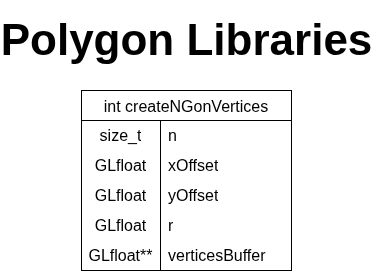
\includegraphics[width=0.7\textwidth]{figures/diagrams/libraries_polygon.png}
    \caption{Diagrama de la biblioteca de polígonos.}
    \label{fig:graph-libraries-polygon}
\end{figure}

\subsection{API pública}
El usuario debería utilizar la función \textit{createNGonVertices} para crear un polígono regular de $n$ vértices, aportando un \textit{buffer} donde almacenarlos y unas coordenadas bidimensionales que servirán de desplazamiento desde el centro de la pantalla.

Una vez calculados los vértices y sus coordenadas queda calcular la distribución de los triángulos dentro de este polígono. Pueden ser representados como un \textit{triangle fan} y exactamente $n-2$ triángulos; en OpenGL se asigna $GL\_TRIANGLE\_FAN$ en la función que dibuja el polígono. El primer vértice actúa de nodo principal y cada pareja de vértices posteriores se conecta al primero.

\section{Animaciones} \label{sec:lib-animation}

En esta sección se trata la biblioteca de \textbf{animaciones} \ref{fig:graph-libraries-animation} su motivación, funciones, estructuras de datos y la \textit{API} pública que ofrece.

Se ha creado esta biblioteca con el propósito de facilitar la animación de geometría, permitiendo mover, escalar y rotar, ya sea cargando de una vez una serie de transformaciones o una a una. Gestiona los fotogramas y la acción en cada uno de ellos, aunque con un alto grado de personalización.

\begin{figure}[htp]
    \begin{subfigure}[t]{1.0\textwidth}
        \centering
        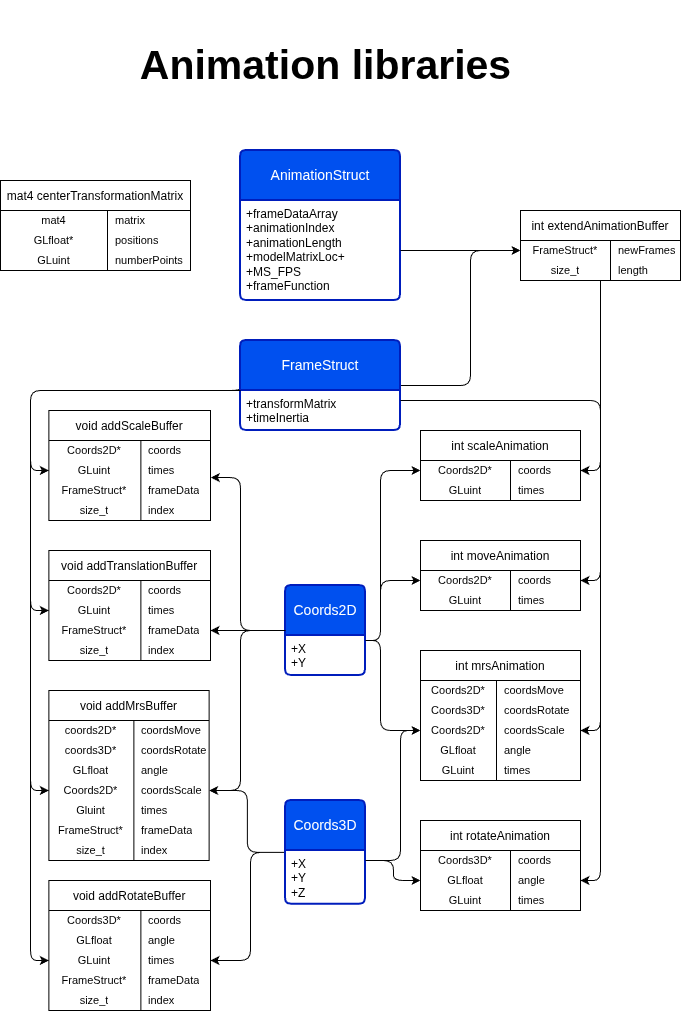
\includegraphics[width=1.0\textwidth]{figures/diagrams/libraries_animation1.png}
        \caption{Diagrama de la biblioteca de animaciones; parte 1.}
        \label{fig:graph-libraries-animation1}
    \end{subfigure}
\end{figure}
    
\begin{figure}[htp]
    \begin{subfigure}[t]{1.0\textwidth}
        \ContinuedFloat
        \centering
        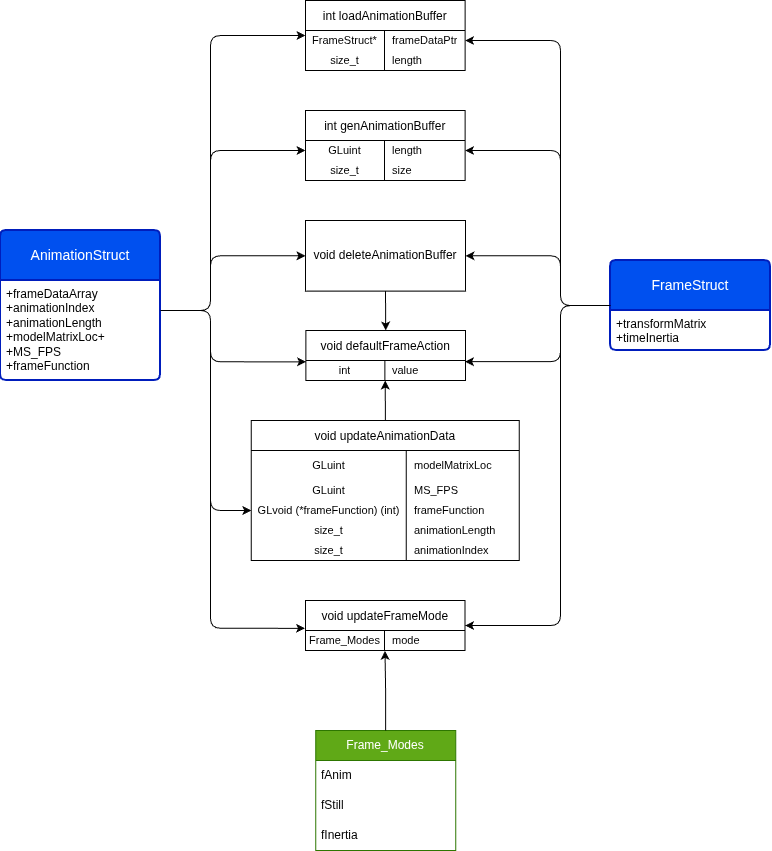
\includegraphics[width=1.0\textwidth]{figures/diagrams/libraries_animation2.png}
        \caption{Diagrama de la biblioteca de animaciones; parte 2.}
        \label{fig:graph-libraries-animation2}
    \end{subfigure}
\caption{Diagrama de la biblioteca de animaciones}
\end{figure} \label{fig:graph-libraries-animation}

\FloatBarrier
\subsection{Decisiones de diseño}

El código \ref{cod:headers-animation-libraries-1} \ref{cod:headers-animation-libraries-2} muestra el prototipo de la biblioteca en código \textit{C}.

La primera parte del diagrama \ref{fig:graph-libraries-animation1} muestra las funciones usadas para transformar la posición de la geometría: 

\begin{itemize}
    \item La estructura \textit{AnimationStruct} describe la animación: fotogramas, número de repeticiones (inercia), \textit{FPS}, etc. Para representar coordenadas, se han creado dos estructuras que describen coordenadas bidimensionales y tridimensionales.

    \item La estructura \textit{FrameStruct} describe las características de un fotograma: la matriz de transformación asociada y el tiempo de inercia, que es el número de veces que se repetirá dicha transformación.

    \item Las estructuras \textit{Coords2D} y \textit{Coords3D} almacenan coordenadas bidimensionales y tridimensionales, respectivamente, en formato decimal
    
    \item Las funciones a la izquierda modifican un \textit{buffer} local, usado más tarde para cargarlo en la animación: 
    
    \begin{enumerate}
        \item La función \textit{addScaleBuffer} agrega a un \textit{buffer} una matriz de transformación de escala.
        
        \item La función \textit{addTranslationBuffer} agrega a un \textit{buffer} una matriz de transformación de desplazamiento.
        
        \item La función \textit{addMrsBuffer} agrega a un \textit{buffer} una matriz de transformación de escala, desplazamiento y rotación, combinados.
        
        \item La función \textit{addRotateBuffer} agrega a un \textit{buffer} una matriz de transformación de rotación.
    \end{enumerate}
    
    \item Las funciones de la derecha modifican directamente la animación sin intermediario, lo que es más sencillo aunque costoso. También, debe estar configurada correctamente la animación antes de utilizarlas.
    
    \begin{enumerate}
        \item La función \textit{scaleAnimation} agrega al \textit{buffer} de animación directamente una matriz de transformación de escala.
        
        \item La función \textit{moveAnimation} agrega al \textit{buffer} de animación directamente una matriz de transformación de desplazamiento.
        
        \item La función \textit{mrsAnimation} agrega al \textit{buffer} de animación directamente una matriz de transformación de escala, desplazamiento y rotación, combinados.
        
        \item La función \textit{rotateAnimation} agrega al \textit{buffer} de animación directamente una matriz de transformación de rotación.
    \end{enumerate}
    
\end{itemize}

La segunda parte del diagrama \ref{fig:graph-libraries-animation2} muestra las funciones relacionadas a la configuración y las acciones de cada fotograma; concretamente, trata la configuración previa a la animación así como la limpieza posterior.

\begin{itemize}
    \item El enumerado, llamado \textit{Frame\_Modes}, contiene 3 estados: quieto, animación e inercia. Cuando no está en movimiento, está \textbf{quieto}; cuando está en movimiento, está en \textbf{animación}; cuando sigue repitiéndose el movimiento, está en \textbf{inercia}, hasta que para y vuelve a \textbf{quieto}.

    \item La función \textit{updateAnimationData} inicializa las propiedades de la animación almacenadas en una estructura \textit{AnimationStruct} global.

    \item El trío de funciones \textit{genAnimationBuffer}, \textit{loadAnimationBuffer} y \textit{deleteAnimationBuffer} trata el ciclo de vida de la animación: crea espacio inicial para la animación, deposita fotogramas y finalmente las destruye, respectivamente.
    
    \item La función \textit{defaultFrameAction} indica lo que ocurre en cada fotograma. Por defecto, se selecciona una función ya existente que aplica las matrices de transformación cada fotograma tantas veces como se indique en el tiempo de inercia y avanza hacia el siguiente.

    \item Finalmente, la función \textit{updateFrameMode} actualiza el estado de la animación y prepara un temporizador que activa el siguiente fotograma.
\end{itemize}

\lstinputlisting[
    float,
    floatplacement=htp,
    language=C,
    label=cod:headers-animation-libraries-1,
    caption=Prototipos de la bibliteca de animación; parte 1,
]{code/h_animation_libraries_1.h}

\lstinputlisting[
    float,
    floatplacement=htp,
    language=C,
    label=cod:headers-animation-libraries-2,
    caption=Prototipos de la biblioteca de animación; parte 2
]{code/h_animation_libraries_2.h}

\FloatBarrier
\subsection{API pública}
El usuario, según la manera en la que desee cargar los fotogramas de la animación, deberá utilizar las funciones que operan directamente sobre el \textit{buffer} de animación o las que tratan primero con un \textit{buffer} local para luego cargarlas en la animación.

En la primera opción, se asigna primero espacio en memoria al \textit{buffer} de animación y se inicializa \textit{AnimationStruct} mediante la función \textit{updateAnimationData}. Luego, se crean listas de coordenadas \textit{Coords2D} y \textit{Coords3D} para ser usadas en las transformaciones y listas de fotogramas \textit{FrameStruct}. Después, se programa la animación con las funciones \textit{add*Buffer}, cargándolas en memoria mediante \textit{loadAnimationBuffer}. Opcionalmente, puede extenderse la animación repitiendo el proceso o usando las funciones \textit{rotate|scale|moveAnimation}.

Si no se desea cargar la animación de la primera forma, sólo se modificaría la llamada a \textit{genAnimationBuffer}, indicando que el tamaño sería \textbf{cero}, y no se usarían las funciones \textit{add*Buffer} y \textit{loadAnimationBuffer}.

